\documentclass[nobib]{tufte-handout}

%\\geometry{showframe}% for debugging purposes -- displays the margins

\newcommand{\bra}[1]{\left(#1\right)}
\usepackage{hyperref}
\usepackage[activate={true,nocompatibility},final,tracking=true,kerning=true,spacing=true,factor=1100,stretch=10,shrink=10]{microtype}
\usepackage{color}

% Fixes captions and images being cut off
\usepackage{marginfix}

\usepackage{pgfplots}
\usepackage[americancurrents, americaninductors, americanvoltages, americanresistors]{circuitikz}
\usepackage{siunitx}
\usepackage{amsmath,amsthm}
\usetikzlibrary{shapes}
\usetikzlibrary{positioning}
\usetikzlibrary{arrows}

% Set up the images/graphics package
\usepackage{graphicx}
\setkeys{Gin}{width=\linewidth,totalheight=\textheight,keepaspectratio}
\graphicspath{{.}}

\title{Notes for ECE 30500 - Semiconductor Devices}
\author[Shubham Saluja Kumar Agarwal]{Shubham Saluja Kumar Agarwal}
\date{\today}  % if the \date{} command is left out, the current date will be used

% The following package makes prettier tables.  We're all about the bling!
\usepackage{booktabs}

% The fancyvrb package lets us customize the formatting of verbatim
% environments.  We use a slightly smaller font.
\usepackage{fancyvrb}
\fvset{fontsize=\normalsize}

% Small sections of multiple columns
\usepackage{multicol}

% These commands are used to pretty-print LaTeX commands
\newcommand{\doccmd}[1]{\texttt{\textbackslash#1}}% command name -- adds backslash automatically
\newcommand{\docopt}[1]{\ensuremath{\langle}\textrm{\textit{#1}}\ensuremath{\rangle}}% optional command argument
\newcommand{\docarg}[1]{\textrm{\textit{#1}}}% (required) command argument
\newenvironment{docspec}{\begin{quote}\noindent}{\end{quote}}% command specification environment
\newcommand{\docenv}[1]{\textsf{#1}}% environment name
\newcommand{\docpkg}[1]{\texttt{#1}}% package name
\newcommand{\doccls}[1]{\texttt{#1}}% document class name
\newcommand{\docclsopt}[1]{\texttt{#1}}% document class option name

% Define a custom command for definitions
\newcommand{\defn}[2]{\noindent\textbf{#1}:\ #2}

\begin{document}

\maketitle

\begin{abstract}
    These are lecture notes for Fall 2025 ECE 30500 by professor Haitong Li at Purdue. Modify, use, and distribute as you please.
\end{abstract}

\tableofcontents

\newpage

\section{Properties of Silicon}
The core of semiconductors lies in the silicon transistor. But, why silicon (\textbf{Si})?\\
\begin{itemize}
    \item Si is the second most common element on Earth.
    \item It is easily purified, and grown defect free, with less than 1 impurity in $10^9$ atoms.
    \item Reasonably good electronic properties
    \item Resilient to harsh environments
    \item Excellent mechanical properties
    \item There are three forms of Si: \begin{itemize}
        \item In a Si crystal, atoms are arranged in an orderly array, allowing arrangements to be easily reproduced.
        \item In poly-crystalline Si, many crystalline subsections exist.
        \item In amorphous Si, there are no long range patterns or arrangements.
    \end{itemize}
\end{itemize}
The unit cell is a portion of any crystal that could be used to reproduce the crystal.\\
The primitive cell is the smallest possible unit cell.\\
In essence, a unit cell is a subset of a lattice that can be moved in the x, y, z axis, and cover the entire lattice. (\textit{Note the absence of rotation movements.})\\
Some examples of cells are the following:
\begin{center}
    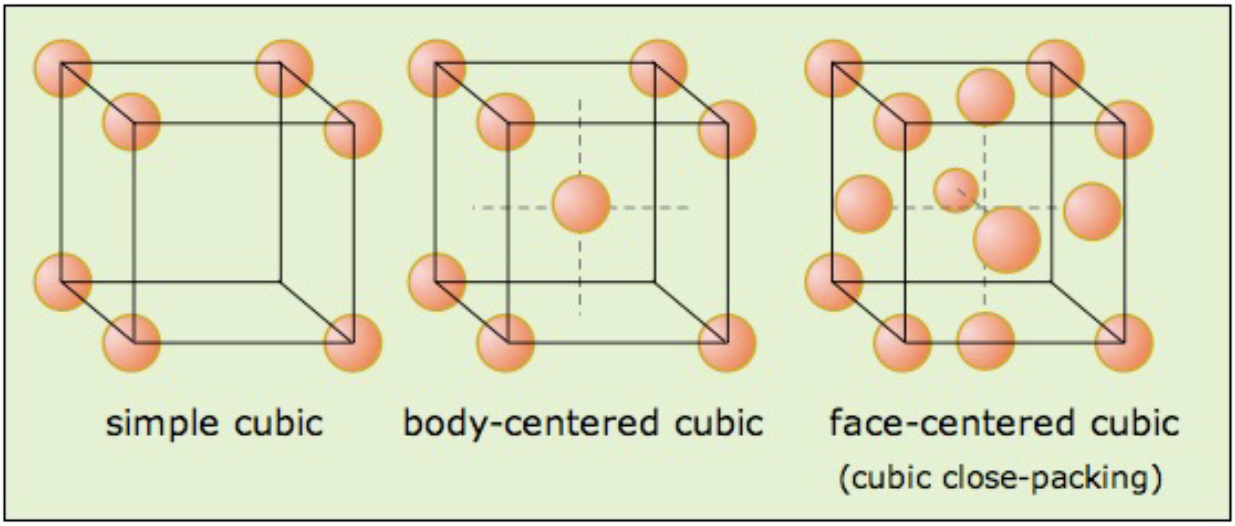
\includegraphics[width = 250px]{images/unit_cell_cube.png}
\end{center}
\textit{Note: the image is missing a corner atom.}\\
Another important cubic unit cell is the diamond cubic unit cell with 8 silicon atoms in the cell:
\begin{center}
    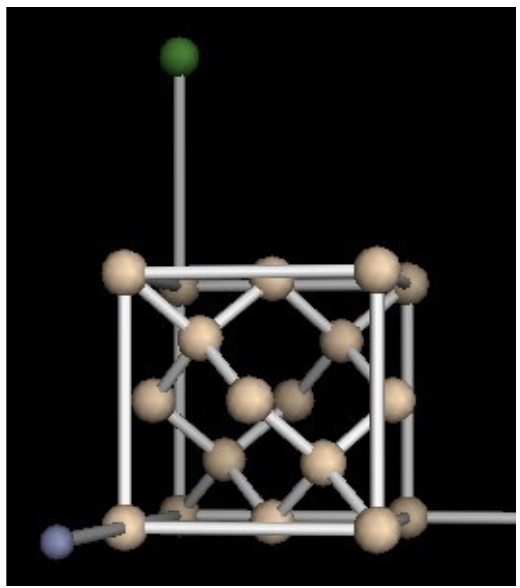
\includegraphics[width = 175px]{images/diamond_cube_cell.png}
\end{center}
\subsection{Density (diamond cube cell)}
Lattice constant: $a=5.3407Ang$\\
Atomic mass: $28.055$amu\\
Density: $\rho = \frac{8*28.0855*1.6605*10^{-23}}{(5.4307*10^{-10})^3}kg/m^3 = 2.3296g/cm^3$
\subsection{Miller Indices}
Let us consider a plane that intercepts the axes at $x_{int}, y_{int}, z_{int}$.
The equation of the plane is:
\begin{equation*}
    \frac{x}{x_{int}}+\frac{y}{y_{int}}+\frac{z}{z_{int}} = 1
\end{equation*}
The vector that is perpendicular to this plane will have the same components as the Miller indices.\\
The Miller indices are defined as $LCM*(\frac{1}{x_{int}},\frac{1}{y_{int}},\frac{1}{z_{int}})$.
\end{document}
